\chapter{Αποτελέσματα Αξιολόγησης}
\label{ch:experiments}

\section{Κλειστός Βρόχος --- Teacher-Forcing (CL/TF)}
\label{sec:cl_results}

\subsection{Αποτελέσματα 1 Μήνα (Δεκέμβριος 2025)}

Στον Πίνακα~\ref{tab:cl_price_1m} παρουσιάζονται τα αποτελέσματα για την πρόβλεψη τιμής DAM
με teacher-forcing για τον Δεκέμβριο 2025. Η εκπαίδευση έγινε με δεδομένα έως 30 Νοε.\ 2025.

\begin{table}[H]
\centering
\caption{Αποτελέσματα Κλειστού Βρόχου (TF) -- Τιμή, Δεκ.\ 2025 (744h).}
\label{tab:cl_price_1m}
\begin{tabular}{lcccc}
\toprule
\textbf{Μοντέλο} & \textbf{MAE (€/MWh)} & \textbf{RMSE (€)} & \textbf{sMAPE (\%)} & \textbf{Κατάταξη} \\
\midrule
Ensemble-Best3 (1/MAE) & \textbf{9,943} & --- & --- & 1 \\
XGBoost & 10,204 & 16,170 & 11,087 & 2 \\
LightGBM & 10,334 & 16,236 & 11,178 & 3 \\
RandomForest & 11,220 & 18,206 & 11,467 & 4 \\
MLP-Optuna & 11,686 & 17,498 & 12,108 & 5 \\
SVR & 13,432 & 19,070 & 13,666 & 6 \\
\midrule
Naive-1 (baseline) & 13,709 & 22,748 & 13,013 & --- \\
Seasonal Profile & 21,524 & 32,157 & 18,389 & --- \\
\bottomrule
\end{tabular}
\end{table}

\begin{table}[H]
\centering
\caption{Αποτελέσματα Κλειστού Βρόχου (TF) -- Φορτίο, Δεκ.\ 2025 (744h).}
\label{tab:cl_load_1m}
\begin{tabular}{lccc}
\toprule
\textbf{Μοντέλο} & \textbf{MAE (MW)} & \textbf{RMSE (MW)} & \textbf{sMAPE (\%)} \\
\midrule
Ensemble-Best3 (1/MAE) & \textbf{72,916} & --- & --- \\
XGBoost & 75,885 & --- & --- \\
LightGBM & 76,324 & --- & --- \\
MLP-Optuna & 78,992 & --- & --- \\
RandomForest & 96,539 & --- & --- \\
SVR & 141,406 & --- & --- \\
\midrule
Seasonal Profile (baseline) & 233,857 & 297,714 & 4,177 \\
Naive-1 (baseline) & 241,807 & 304,823 & 4,439 \\
\bottomrule
\end{tabular}
\end{table}

\noindent\textbf{Βασικές Παρατηρήσεις:}
\begin{itemize}
    \item Το Ensemble-Best3 (σταθμισμένος 1/MAE μέσος XGB+LGBM+RF) επιτυγχάνει το καλύτερο MAE
    τιμής (9,943 €/MWh), βελτιώνοντας κατά 27\% έναντι του Naive-1 (13,709 €/MWh).
    \item Για φορτίο, το Ensemble-Best3 επιτυγχάνει 72,916 MW, αντιπροσωπεύοντας 70\% βελτίωση
    έναντι Seasonal Profile (233 MW).
    \item Η SVR αποδίδει σημαντικά χειρότερα από τα tree models --- αδυναμία που εντείνεται για
    μεγαλύτερες περιόδους αξιολόγησης.
\end{itemize}

\subsection{Αποτελέσματα Q1 2026 (Δεκ.\ 2025 -- Φεβ.\ 2026)}

Η επέκταση σε τριμηνιαία αξιολόγηση (2160 ώρες) αποκαλύπτει σημαντική αύξηση σφάλματος για
όλα τα μοντέλα, ιδιαίτερα για SVR που αποτυγχάνει παταγωδώς τον Ιανουάριο-Φεβρουάριο 2026:

\begin{table}[H]
\centering
\caption{Αποτελέσματα CL -- Τιμή, Q1 2026 (2160h).}
\label{tab:cl_price_q1}
\begin{tabular}{lcccc}
\toprule
\textbf{Μοντέλο} & \textbf{MAE (€/MWh)} & \textbf{RMSE (€)} & \textbf{sMAPE (\%)} & \textbf{Κατάταξη} \\
\midrule
Ensemble-Best3 & \textbf{14,478} & 22,193 & 25,085 & 1 \\
LightGBM & 14,556 & 22,292 & 25,541 & 2 \\
RandomForest & 15,161 & 23,634 & 25,072 & 3 \\
Naive-1 & 15,433 & 26,781 & 22,635 & --- \\
XGBoost & 15,888 & 23,353 & 26,519 & 4 \\
MLP-Optuna & 17,917 & 25,209 & 28,367 & 5 \\
MLP & 18,707 & 25,136 & 28,722 & 6 \\
SVR & 40,775 & 53,172 & 41,412 & ⚠ \\
\bottomrule
\end{tabular}
\end{table}

Η κατάρρευση της SVR ($\text{MAE}=40,8$ €/MWh) αποδίδεται στη μετατόπιση κατανομής (distribution
shift): εκπαίδευση σε διάστημα 2017--2025 με μέση τιμή $\approx$ 80 €/MWh, αλλά τον Ιανουάριο
2026 η αγορά παρουσιάζει υψηλή μεταβλητότητα άνω των 200 €/MWh.


\section{Ανοικτός Βρόχος --- Recursive (OL)}
\label{sec:ol_results}

\subsection{Δεκέμβριος 2025 (Μηνιαία Αξιολόγηση)}

\begin{table}[H]
\centering
\caption{Open-Loop H=24 (daily) -- Τιμή, Δεκ.\ 2025.}
\label{tab:ol_price_1m}
\begin{tabular}{lcccc}
\toprule
\textbf{Μοντέλο} & \textbf{MAE (€/MWh)} & \textbf{RMSE (€)} & \textbf{Chunks} & \textbf{Κατάταξη} \\
\midrule
Ensemble-Top3 1/MAE & \textbf{13,960} & 21,958 & 24h & 1 \\
LGBM-Daily-Optuna & 14,494 & 22,511 & 24h & 2 \\
RF-Daily-SS & 14,607 & 23,015 & 24h & 3 \\
XGB-Daily-SS-Optuna Dense & 14,816 & --- & 24h & 4 \\
LGBM-Daily-SS-Optuna Dense & 14,744 & --- & 24h & 5 \\
MLP-SS & 15,169 & 22,065 & 24h & 6 \\
XGB-OL-Optuna (weekly) & 17,007 & 26,404 & 168h & 7 \\
SVR-OL & 18,549 & 25,602 & 24h & 8 \\
\midrule
Naive-1 & 14,930 & 25,963 & --- & --- \\
\bottomrule
\end{tabular}
\end{table}

\textbf{Κύρια εύρηματα OL τιμής:}
\begin{itemize}
    \item Τα daily chunks (H=24) υπερτερούν σημαντικά έναντι weekly (H=168): $-16,7\%$ MAE
    (14,494 vs 17,410 €/MWh για LGBM). Η συσσώρευση σφάλματος σε 168 βήματα είναι σημαντικά
    μεγαλύτερη.
    \item Το Ensemble-Top3 (LGBM+RF+XGB, σχεδόν ίσα βάρη $\approx 0.33$) επιτυγχάνει $-19,8\%$
    έναντι εβδομαδιαίου βέλτιστου.
    \item Το SS δεν βοηθάει το LGBM (\texttt{14,494$\to$14,986}, χειρότερο), αλλά βοηθάει το XGB
    (\texttt{15,312$\to$15,036}, βελτίωση). Υπόθεση: LGBM (leaf-wise) είναι ήδη ανθεκτικό, ενώ XGB
    ωφελείται από καλύτερη ρύθμιση.
\end{itemize}

\begin{table}[H]
\centering
\caption{Open-Loop H=24 -- Φορτίο, Δεκ.\ 2025.}
\label{tab:ol_load_1m}
\begin{tabular}{lcc}
\toprule
\textbf{Μοντέλο} & \textbf{MAE (MW)} & \textbf{Κατάταξη} \\
\midrule
LGBM-Daily-SS-Optuna & \textbf{80,704} & 1 \\
XGB-Daily-Optuna & 99,575 & 2 \\
RF-Daily-SS & 117,740 & 3 \\
MLP-SS & 122,604 & 4 \\
SVR-OL & 184,739 & 5 \\
\bottomrule
\end{tabular}
\end{table}

\noindent Για φορτίο, το SS \textit{βοηθάει} το LGBM (80,7 vs $\approx$90 MW για LGBM χωρίς SS),
αντίθετα από ό,τι συμβαίνει με την τιμή.


\section{MIMO (Multi-Input Multi-Output)}
\label{sec:mimo_results}

\begin{table}[H]
\centering
\caption{MIMO H=24 -- Τιμή, Δεκ.\ 2025 (744h, daily prediction).}
\label{tab:mimo_price_1m}
\begin{tabular}{lccc}
\toprule
\textbf{Μοντέλο} & \textbf{MAE (€/MWh)} & \textbf{RMSE (€)} & \textbf{Κατάταξη} \\
\midrule
Ensemble-Best3 1/MAE & \textbf{15,202} & --- & 1 \\
XGB MIMO Dense & 15,503 & 23,896 & 2 \\
LGBM Direct Dense & 15,521 & 24,075 & 3 \\
LGBM Direct+Load (two-stage) & 16,190 & 24,630 & 4 \\
RF MIMO+Load Dense & 16,812 & 25,920 & 5 \\
SVR MIMO+Load Dense & 18,048 & 25,651 & 6 \\
MLP MIMO+Load Dense & 19,966 & 27,652 & 7 \\
\midrule
Seasonal Profile & 18,127 & 27,388 & --- \\
Naive-24 (MIMO context) & 18,213 & --- & --- \\
\bottomrule
\end{tabular}
\end{table}

\begin{table}[H]
\centering
\caption{MIMO H=24 -- Φορτίο, Δεκ.\ 2025 (744h).}
\label{tab:mimo_load_1m}
\begin{tabular}{lccc}
\toprule
\textbf{Μοντέλο} & \textbf{MAE (MW)} & \textbf{RMSE (MW)} & \textbf{Κατάταξη} \\
\midrule
Ensemble-Best3 1/MAE & \textbf{189,005} & --- & 1 \\
XGB MIMO Dense & 190,308 & 295,817 & 2 \\
LGBM Direct Dense & 194,417 & 304,411 & 3 \\
RF MIMO & 219,250 & 313,966 & 4 \\
MLP MIMO & 219,884 & 308,093 & 5 \\
\midrule
Seasonal Profile & 291,557 & 396,534 & --- \\
SVR MIMO (5K rows) & 586,623 & --- & ⚠ \\
\bottomrule
\end{tabular}
\end{table}

\noindent\textbf{Dense Lags και MIMO:} Τα dense intraday lags (lag 3--23) βοηθούν σημαντικά στο
MIMO, διότι κατά την εκπαίδευση MIME χρησιμοποιούνται \textit{πραγματικές} ιστορικές τιμές (όχι
αναδρομικές προβλέψεις), επομένως δεν υπάρχει θόρυβος:
\begin{itemize}
    \item XGB Dense MIMO τιμή: $-7,9\%$ (16,839 $\to$ 15,503 €/MWh)
    \item LGBM Dense Direct τιμή: $-6,5\%$ (16,591 $\to$ 15,521 €/MWh)
    \item MLP Dense MIMO τιμή: $-22,3\%$ (25,710 $\to$ 19,966 €/MWh)
\end{itemize}

Αντίθετα, τα dense lags \textit{βλάπτουν} τα OL μοντέλα (LGBM Dense OL: +2,8\% χειρότερο),
διότι στο recursive inference, οι lags 3--23 υπολογίζονται από θορυβώδεις αναδρομικές προβλέψεις.


\section{Walk-Forward Monthly Retraining (MR)}
\label{sec:mr_results}

Τα αποτελέσματα Monthly Retraining για Q1 2026 (2160 ώρες) παρουσιάζονται στους παρακάτω πίνακες.

\begin{table}[H]
\centering
\caption{Walk-Forward Monthly Retrain -- Τιμή, Q1 2026.}
\label{tab:mr_price_q1}
\begin{tabular}{lcccc}
\toprule
\textbf{Μοντέλο} & \textbf{Στρατηγική} & \textbf{MAE (€/MWh)} & \textbf{RMSE (€)} & \textbf{Κατ.} \\
\midrule
Ensemble-TF-Best3 & TF & \textbf{10,491} & 15,726 & 1 \\
TF-LGBM-MR & TF & \textbf{10,463} & 15,682 & 2 \\
TF-XGB-MR & TF & 10,913 & 16,148 & 3 \\
Naive-1 & Baseline & 12,218 & 20,042 & --- \\
TF-RF-MR & TF & 12,806 & 19,089 & 4 \\
TF-MLP-MR & TF & 15,620 & 22,458 & 5 \\
Rec-XGB-SS-DO-MR & Rec & 18,534 & 27,496 & 6 \\
Rec-XGB-DO-MR & Rec & 18,963 & 28,087 & 7 \\
Rec-LGBM-SS-DO-MR & Rec & 19,005 & 28,281 & 8 \\
\midrule
Seasonal Profile & Baseline & 25,054 & 36,813 & --- \\
\bottomrule
\end{tabular}
\end{table}

\begin{table}[H]
\centering
\caption{Ανάλυση ανά μήνα -- TF Monthly Retrain, τιμή.}
\label{tab:mr_price_monthly}
\begin{tabular}{lccccc}
\toprule
\textbf{Μήνας} & \textbf{TF-LGBM} & \textbf{TF-XGB} & \textbf{TF-RF} & \textbf{TF-MLP} & \textbf{Rec-XGB-SS} \\
\midrule
Δεκ.\ 2025 & 8,607 & 8,708 & 10,945 & 10,483 & 14,229 \\
Ιαν.\ 2026 & 11,228 & 12,567 & 12,161 & 22,078 & 18,071 \\
Φεβ.\ 2026 & 11,670 & 11,524 & 15,582 & 14,156 & 23,814 \\
\textbf{Σύνολο Q1} & \textbf{10,463} & \textbf{10,913} & \textbf{12,806} & \textbf{15,620} & \textbf{18,534} \\
\bottomrule
\end{tabular}
\end{table}

\begin{table}[H]
\centering
\caption{Walk-Forward Monthly Retrain -- Φορτίο, Q1 2026.}
\label{tab:mr_load_q1}
\begin{tabular}{lcccc}
\toprule
\textbf{Μοντέλο} & \textbf{Στρατηγική} & \textbf{MAE (MW)} & \textbf{RMSE (MW)} & \textbf{Κατ.} \\
\midrule
Ensemble-TF-Best3 & TF & \textbf{67,729} & 89,324 & 1 \\
TF-LGBM-MR & TF & 69,435 & 92,490 & 2 \\
Rec-XGB-SS-DO-MR & Rec & 70,641 & 93,179 & 3 \\
TF-XGB-MR & TF & 72,925 & 95,540 & 4 \\
Rec-LGBM-SS-DO-MR & Rec & 72,573 & 95,902 & 5 \\
TF-MLP-MR & TF & 88,493 & 116,316 & 6 \\
TF-RF-MR & TF & 100,177 & 136,509 & 7 \\
\bottomrule
\end{tabular}
\end{table}

\noindent\textbf{Κύριο εύρημα:} Η μηνιαία επανεκπαίδευση μειώνει το MAE:
\begin{itemize}
    \item Τιμή: $14,478 \rightarrow 10,463$ €/MWh ($-27,7\%$) έναντι στατικής CL εκπαίδευσης.
    \item Φορτίο: $96,751 \rightarrow 67,729$ MW ($-30,0\%$).
\end{itemize}

Εξαιρετικά σημαντικό εύρημα: για φορτίο, η Rec-XGB-SS-DO-MR (70,641 MW) σχεδόν εξισώνεται
με το TF-LGBM-MR (69,435 MW). Αυτό δείχνει ότι η συσσώρευση σφάλματος είναι πολύ μικρότερη
για φορτίο απ' ό,τι για τιμή, λόγω της φύσεως ομαλότητας.


\section{Σύγκριση Στρατηγικών}
\label{sec:strategy_comparison}

\begin{table}[H]
\centering
\caption{Συγκεντρωτική σύγκριση βέλτιστων μοντέλων ανά στρατηγική.}
\label{tab:strategy_summary}
\begin{tabular}{lcccc}
\toprule
\textbf{Στρατηγική} & \multicolumn{2}{c}{\textbf{Τιμή MAE (€/MWh)}} & \multicolumn{2}{c}{\textbf{Φορτίο MAE (MW)}} \\
\cmidrule(lr){2-3} \cmidrule(lr){4-5}
& Dec'25 & Q1'26 & Dec'25 & Q1'26 \\
\midrule
TF/CL Ensemble-Best3 & 9,943 & 14,478 & 72,916 & 96,751 \\
OL Ensemble-Top3 & 13,960 & 20,094 & 80,704 & 102,961 \\
MIMO Ensemble-Best3 & 15,202 & 20,896 & 189,005 & 217,088 \\
\textbf{MR TF Ensemble-Best3} & \textbf{---} & \textbf{10,491} & \textbf{---} & \textbf{67,729} \\
Naive-1 & 14,930 & 15,433 & 241,807 & --- \\
\bottomrule
\end{tabular}
\end{table}

\noindent Από τον Πίνακα~\ref{tab:strategy_summary} προκύπτουν τα εξής:

\begin{enumerate}
    \item \textbf{TF/CL > OL > MIMO} για τιμή: Η teacher-forcing στρατηγική υπερτερεί σαφώς,
    επιβεβαιώνοντας ότι ο βασικός περιοριστικός παράγοντας για OL/MIMO είναι η απουσία πρόσβασης
    στις πραγματικές lagged τιμές κατά την πρόβλεψη.

    \item \textbf{CL ≈ OL για φορτίο:} Η διαφορά TF vs OL είναι μικρή για φορτίο
    ($+10,7\%$ Dec, $+6,4\%$ Q1), σε αντίθεση με τιμή ($+40,4\%$ Dec, $+38,8\%$ Q1).

    \item \textbf{Monthly Retraining:} Η πλέον αποδοτική στρατηγική για μεγάλους ορίζοντες
    (3 μήνες), μειώνοντας σημαντικά τις επιπτώσεις της αλλαγής κατανομής.

    \item \textbf{Daily (H=24) >> Weekly (H=168) για OL:} Η ημερήσια αξιολόγηση μειώνει δραματικά
    το σφάλμα έναντι της εβδομαδιαίας ($-16,7\%$ για τιμή Dec) λόγω μικρότερης συσσώρευσης.
\end{enumerate}

\begin{figure}[H]
    \centering
    \includegraphics[width=0.9\textwidth]{../thesis_output/ch6_forecast_analysis/01_ts_price.png}
    \caption{Χρονοσειρές προβλέψεων τιμής DAM για επιλεγμένα μοντέλα, Q1 2026.
    Οι αποχρώσεις αντιπροσωπεύουν διαφορετικές στρατηγικές (TF: μοβ, CL: γαλάζιο,
    OL: πράσινο, MIMO: πορτοκαλί).}
    \label{fig:ts_price}
\end{figure}

\begin{figure}[H]
    \centering
    \includegraphics[width=0.9\textwidth]{../thesis_output/ch6_forecast_analysis/02_ts_load.png}
    \caption{Χρονοσειρές προβλέψεων φορτίου για επιλεγμένα μοντέλα, Q1 2026.}
    \label{fig:ts_load}
\end{figure}

\begin{figure}[H]
    \centering
    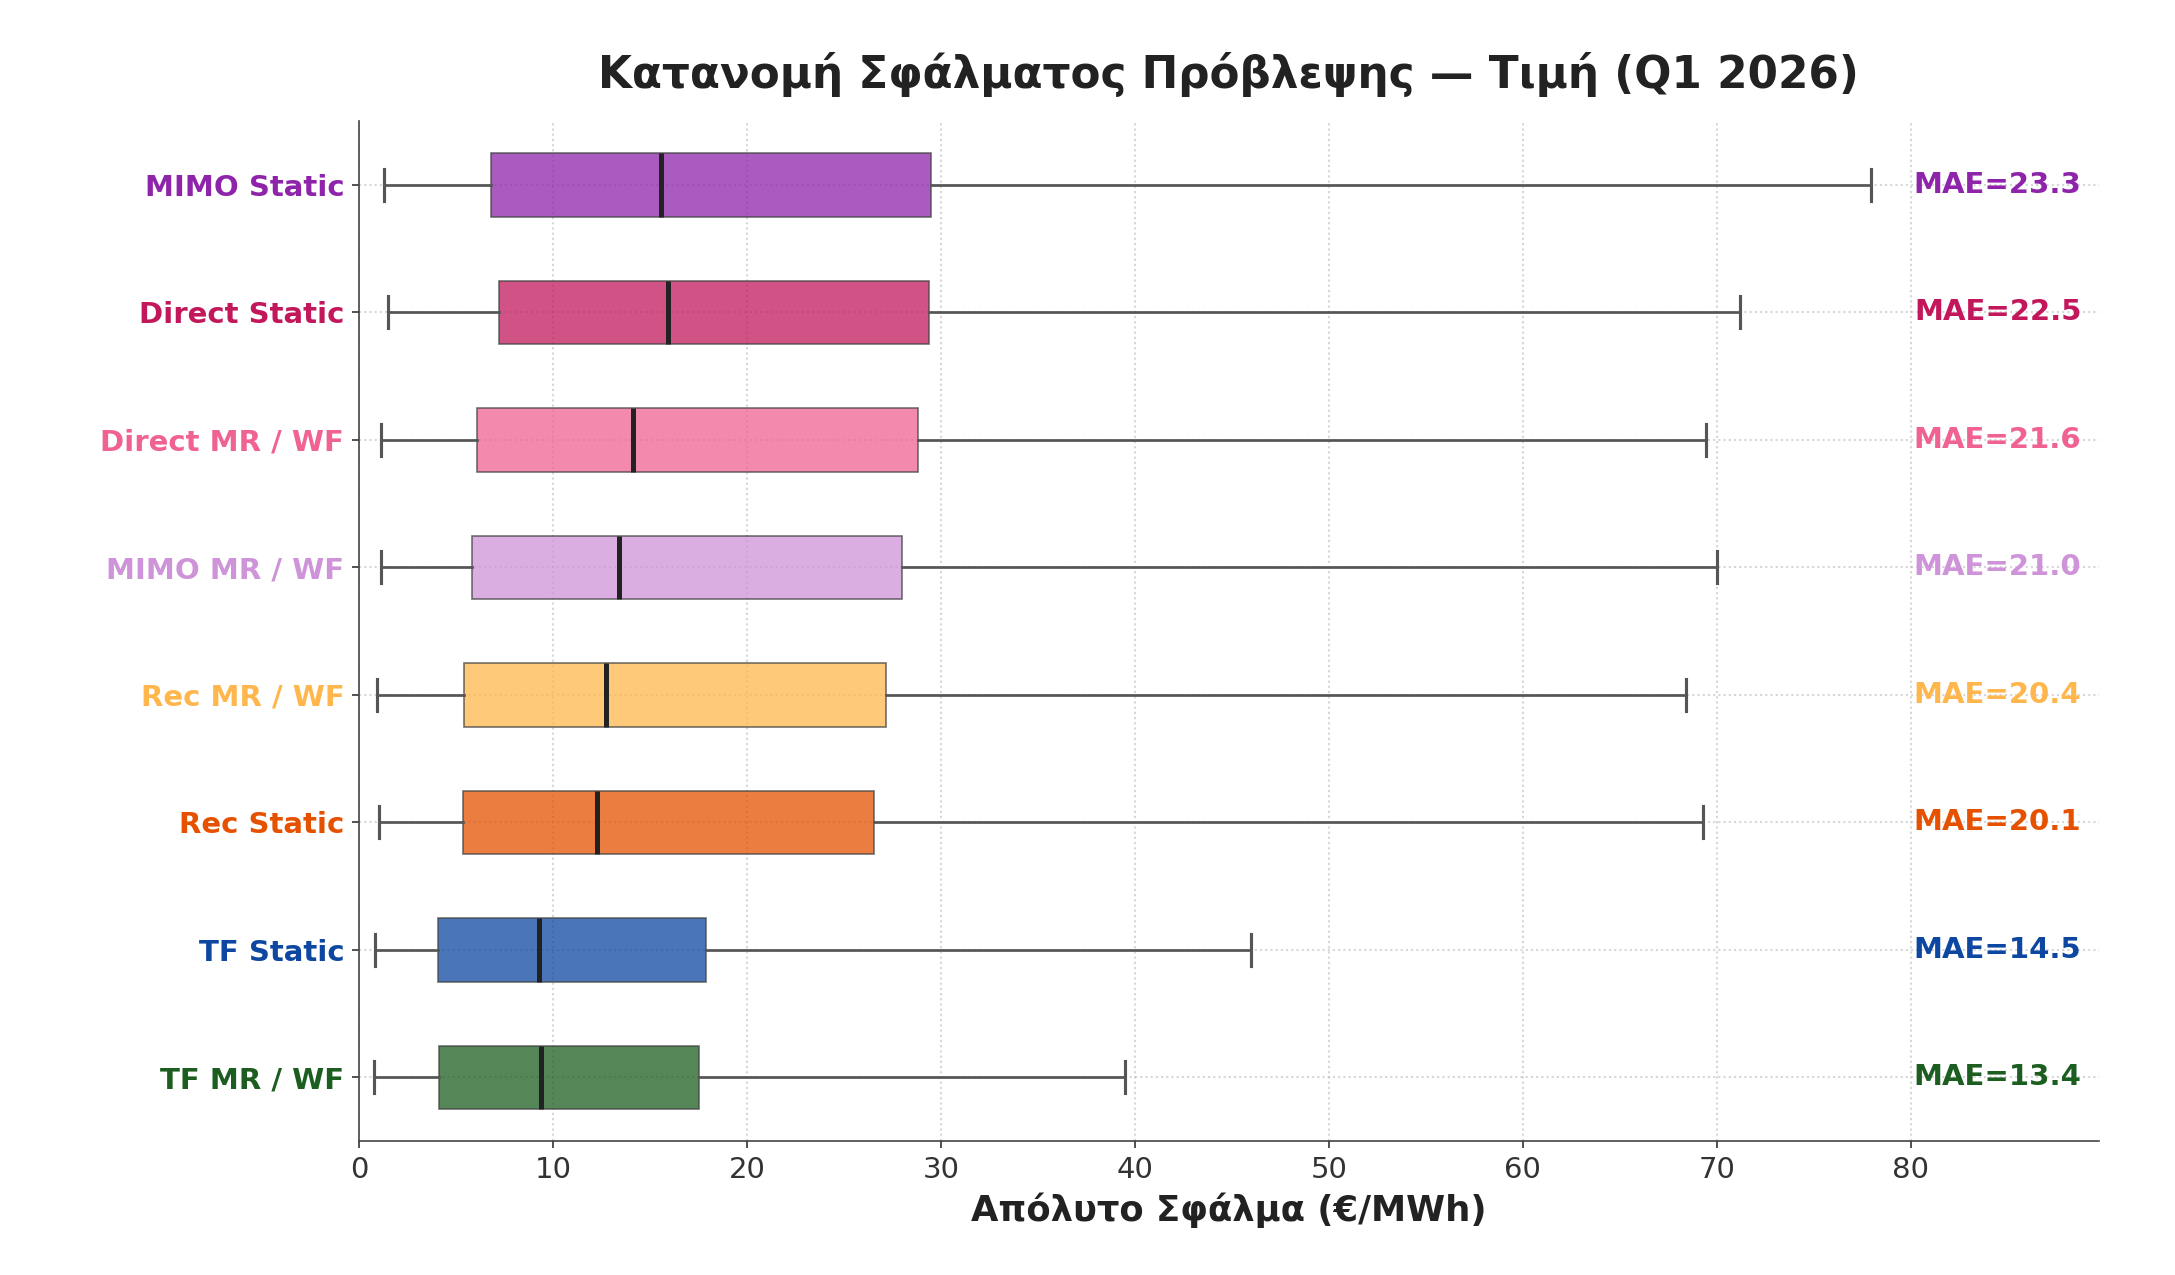
\includegraphics[width=0.9\textwidth]{../thesis_output/ch6_forecast_analysis/05_boxplot_price.png}
    \caption{Box plots κατανομής σφαλμάτων (absolute error) ανά μοντέλο για τιμή, Q1 2026.
    Ο διάμεσος, IQR και outliers αποκαλύπτουν διαφορές στη συνέπεια των μοντέλων.}
    \label{fig:boxplot_price}
\end{figure}

\begin{figure}[H]
    \centering
    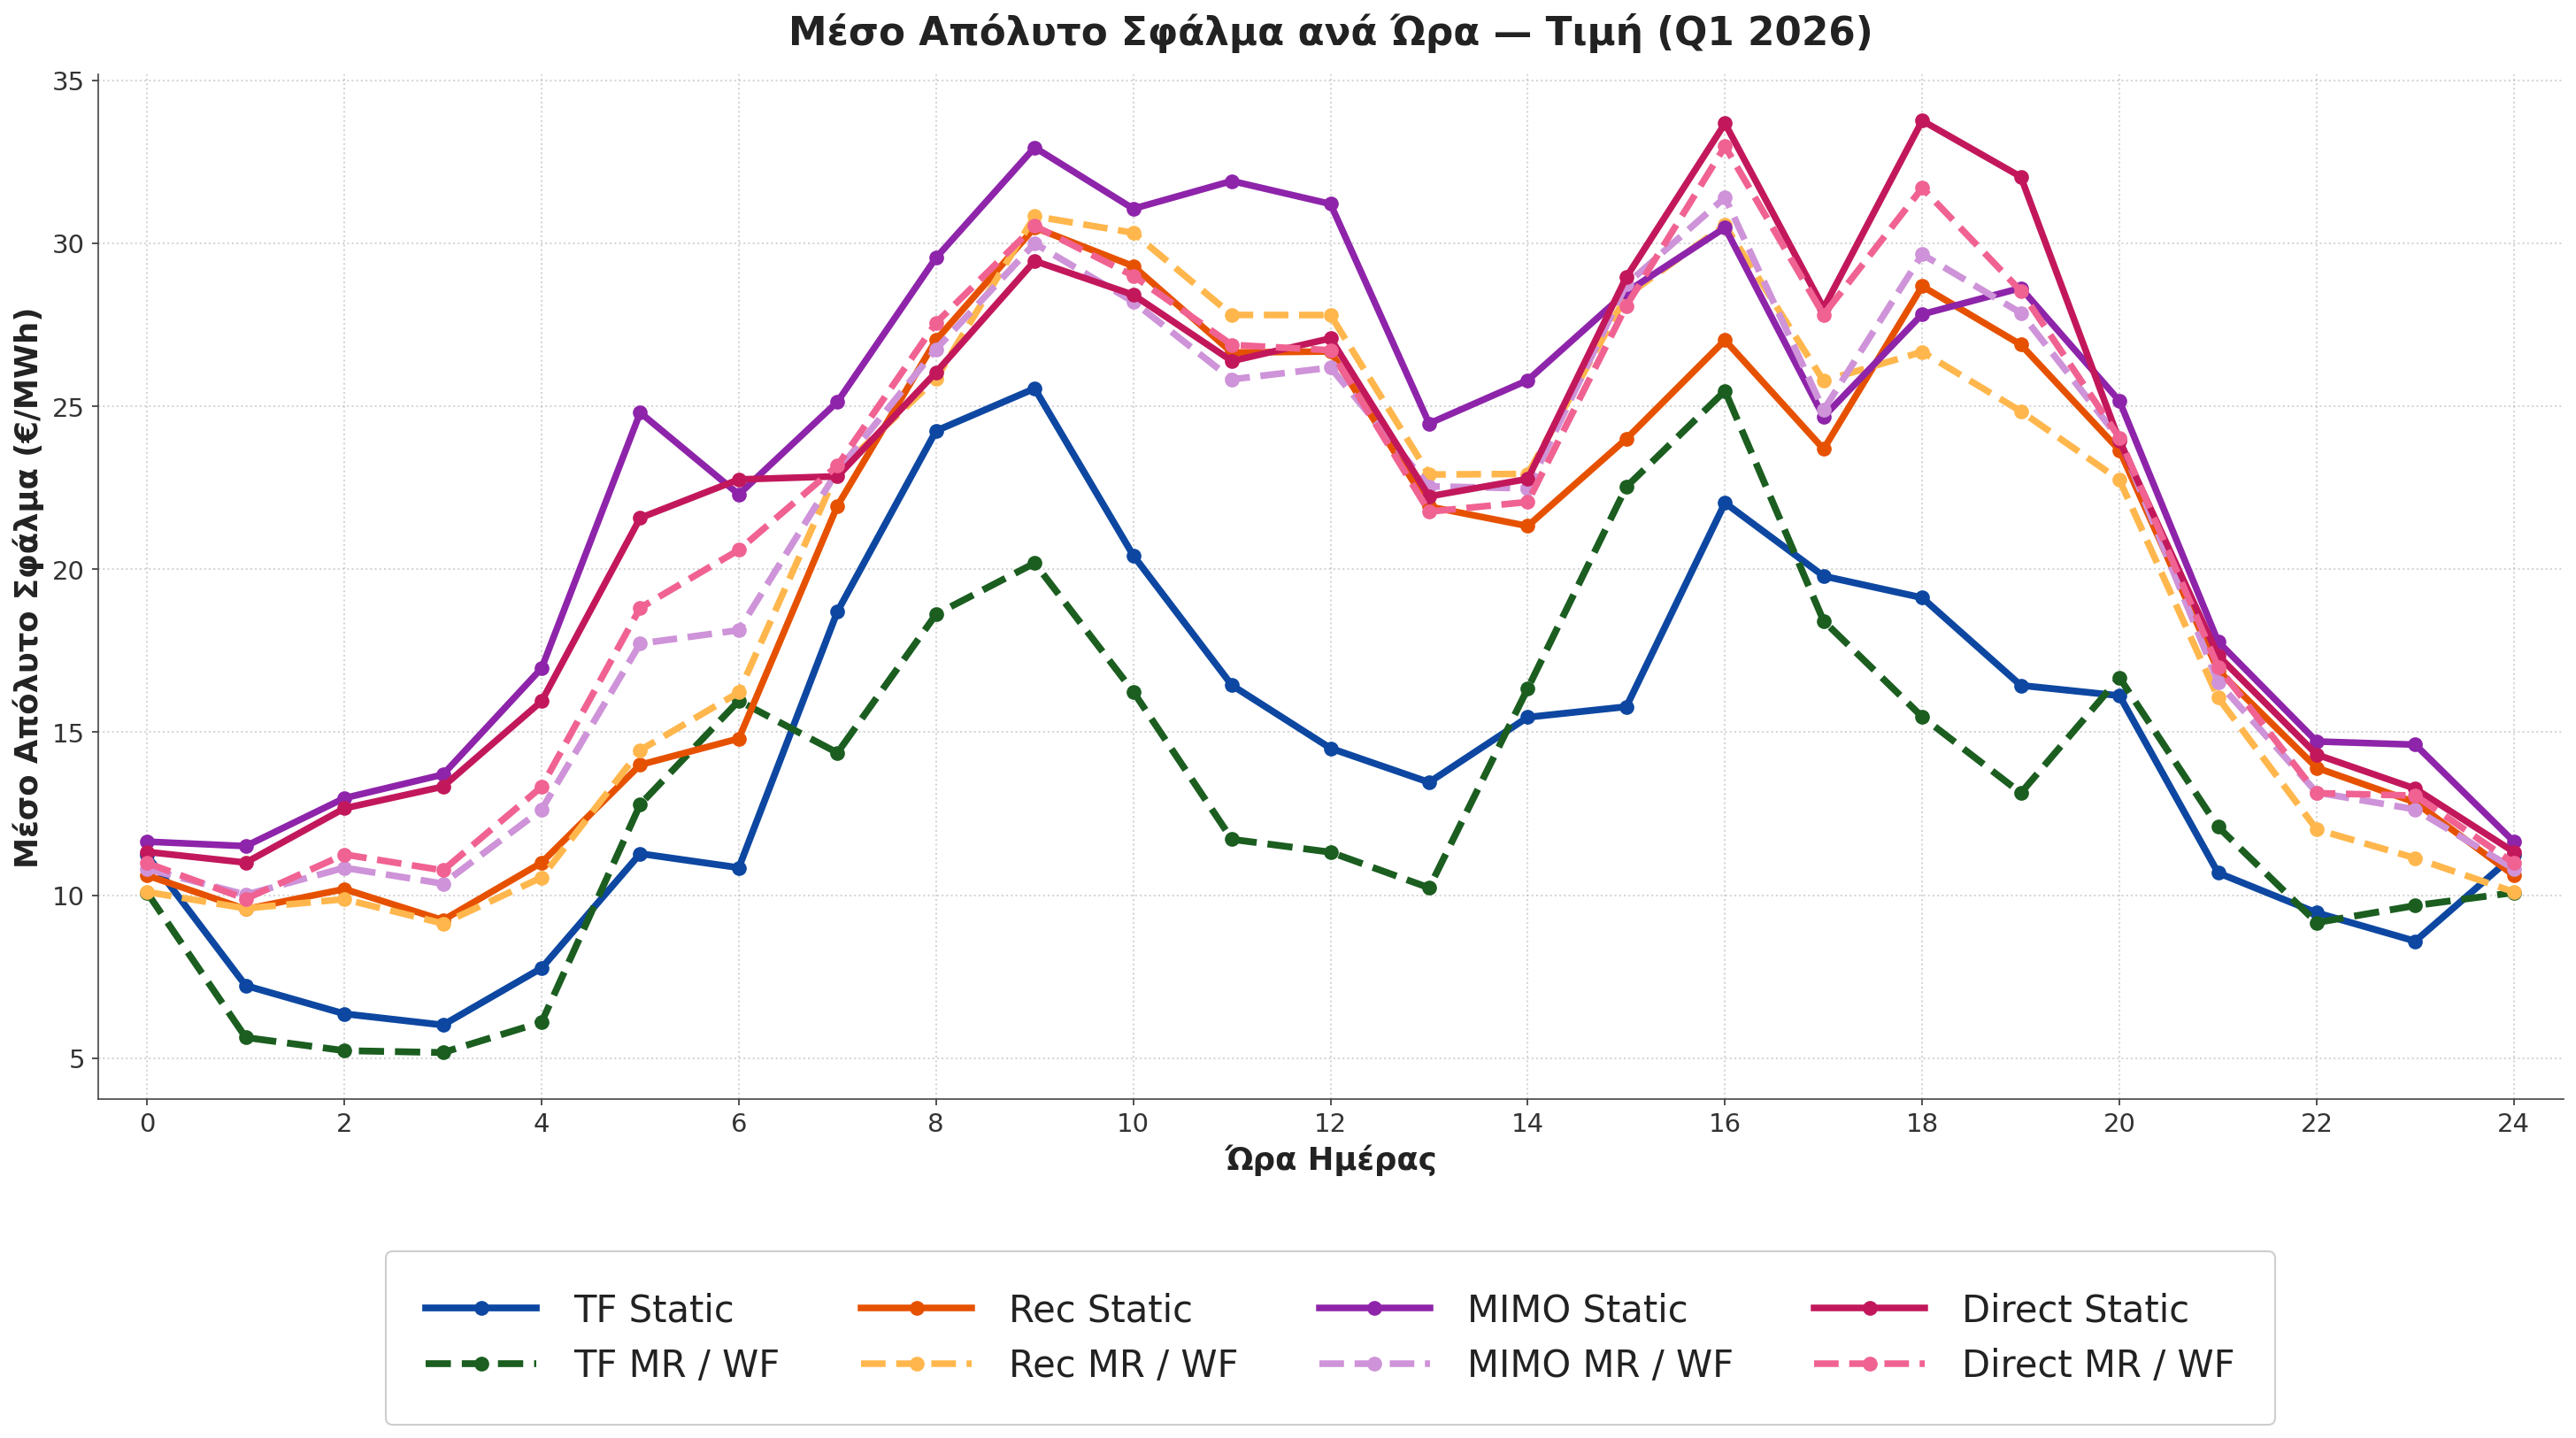
\includegraphics[width=0.9\textwidth]{../thesis_output/ch6_forecast_analysis/07_hourly_price.png}
    \caption{Ωριαίο προφίλ σφάλματος (MAE ανά ώρα ημέρας) για τιμή, Q1 2026.
    Τα μοντέλα δυσκολεύονται ιδιαίτερα τις ώρες αιχμής (19:00--22:00).}
    \label{fig:hourly_price}
\end{figure}
